% !TeX spellcheck = en_US
\documentclass[11pt]{article}
\usepackage{amsmath}
\usepackage{steinmetz}
\usepackage{graphicx}
\usepackage{lipsum}
\usepackage{hyperref}
\usepackage[margin=2cm]{geometry}


\setlength\parindent{0pt}
%opening
\title{Configuraciones especiales y filtros activos}
\author{Juan Barbosa - 201325901}

\begin{document}

\maketitle

\section{Derivador}
Para una capacitancia, se define la impedancia como $Z_c = 1/j\omega c$. Teniendo en cuenta que existe realimentaci\'on negativa, la corriente por la capacitancia es la misma que pasa sobre la resistencia.
\begin{equation}
	\dfrac{V_{in}-V_N}{Z_c} = \dfrac{V_N-V_{out}}{R}
\end{equation}

\noindent como $V_N=V_P=0$
\begin{equation}
	V_{out}=-\dfrac{R}{Z_c}V_{in}=-j\omega RCV_{in}=-RC\dfrac{dV_{in}}{dt}
\end{equation}

\section{Integrador}
De forma an\'aloga, la corriente sobre la resistencia es la misma que atraviesa la capacitancia.
\begin{equation}
	\dfrac{V_{in}-V_N}{R} = \dfrac{V_N-V_{out}}{Z_c}
\end{equation}

\noindent dado que $V_N=V_P=0$
\begin{equation}
	V_{out}=-\dfrac{Z_c}{R}V_{in}=-\dfrac{1}{j\omega RC}V_{in}=-\dfrac{1}{RC}\int V_{in} dt
\end{equation}

\section{Filtro con amplificaci\'on}
Teniendo en cuenta que $C_1$ y $R_1$ est\'an en serie:
\begin{equation}
	Z_{eq} = Z_{c1} + R_1=\dfrac{1+j\omega R_1C}{j\omega C}
\end{equation}

\noindent A partir de los mismos argumentos anteriores,
\begin{equation*}
	\dfrac{V_{in}-V_N}{Z_{eq}}=\dfrac{V_N-V_{out}}{R_2}
\end{equation*}
\begin{equation}
	V_{out} = -\dfrac{R_2}{Z_{eq}}V_{in} = -\dfrac{j\omega R_2C}{1+j\omega R_1C} V_{in}
\end{equation}

\noindent Lo cual se puede escribir en notaci\'on fasorial como:
\begin{equation}
	V_{out} = \dfrac{C R_{2}\omega}{\sqrt{C^{2} R_{1}^{2} \omega^{2} + 1}} V_{in}\phase{\arctan\left(\dfrac{1}{R_1C\omega}\right)}
\end{equation}

\noindent La frecuencia de corte es entonces:
\begin{equation}
	\omega_c = \dfrac{1}{R_1C} \approx 1000 \text{ rad/s}
\end{equation}

\pagebreak
\begin{figure}[h]
	\centering
	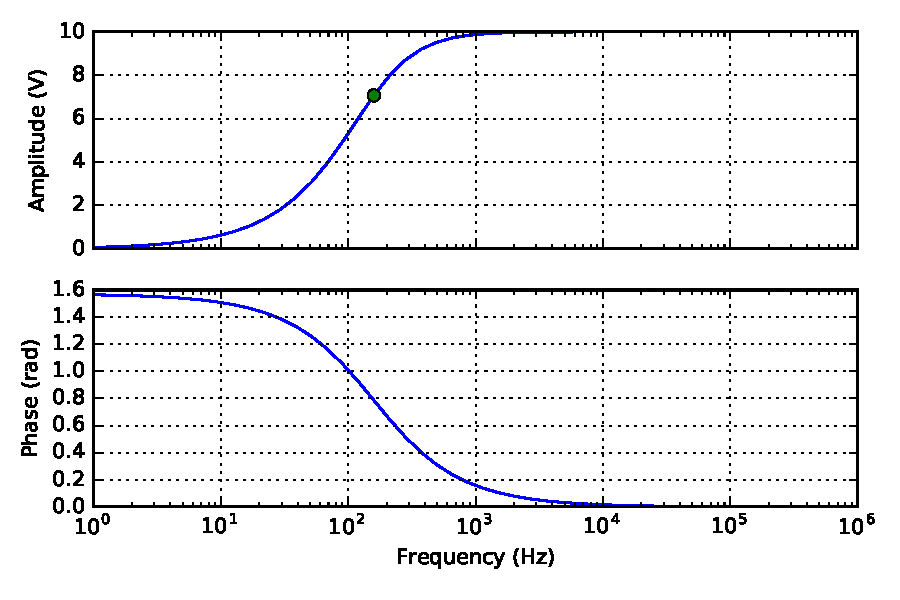
\includegraphics[width=0.5\linewidth]{filter.pdf}
	\caption{Amplitude and phase dependency with the frequency.}
\end{figure}

\section{Filtro pasabanda}
\begin{figure}[h]
	\centering
	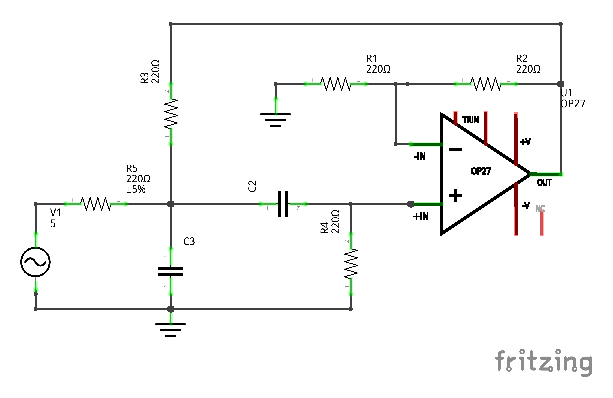
\includegraphics[width=0.5\linewidth]{band-pass.pdf}
	\caption{Currents in the circuit.}
\end{figure}

Las resistencias R4 y R5 forman un divisor de voltaje:
\begin{equation}
	V_N=\dfrac{R_4}{R_4+R_5}V_{out} = V_P
\end{equation}

Sobre el nodo principal se tiene:
\begin{equation}\label{eq:principalNode}
	I_1=I_2+I_3+I_4 \qquad I_4=I_5
\end{equation}

Usando la relaci\'on entre las corrientes I4 e I5, y nombrando como V1 el potencial del nodo principal:
\begin{equation*}
	\dfrac{V_1-V_P}{Z_{c2}} = \dfrac{V_P}{R_2}
\end{equation*}
\begin{equation}
	V_1=V_P\left(\dfrac{Z_{c2}}{R_2}+1\right)=\left(\dfrac{R_4}{R_4+R_5}\right)\left(\dfrac{Z_{c2}}{R_2}+1\right)V_{out}
\end{equation}

Reescribiendo la ecuaci\'on \ref{eq:principalNode} en t\'erminos de potencial:
\begin{equation}
	\dfrac{1}{R_{1}} \left( V_{in} -  V_{1}\right) = \frac{V_{1}}{Z_{c1}} + \frac{1}{R_{3}} \left(V_{1} - V_{out}\right) + \frac{1}{Z_{c2}} \left(V_{1}- \frac{R_{4} V_{out}}{R_{4} + R_{5}}\right)
\end{equation}

Despejando $V_{out}$:
\small
\begin{equation*}
	V_{out}=\frac{R_{2} R_{3} Z_{c1} \left(R_{4} + R_{5}\right)}{R_{1} R_{2} R_{3} R_{4} - R_{1} R_{2} R_{5} Z_{c1} + R_{1} R_{3} R_{4} Z_{c1} + R_{1} R_{3} R_{4} Z_{c2} + R_{1} R_{4} Z_{c1} Z_{c2} + R_{2} R_{3} R_{4} Z_{c1} + R_{3} R_{4} Z_{c1} Z_{c2}}V_{in}
\end{equation*}
\normalsize

Haciendo R1 = R2 = R3, y C1 = C2
\begin{equation}
	\begin{array}{rl}	
	V_{out} & =\dfrac{R_{1}^{2} Z_{c1} \left(R_{4} + R_{5}\right)}{R_{1}^{3} R_{4} + 2 R_{1}^{2} R_{4} Z_{c1} + R_{1}^{2} R_{4} Z_{c2} - R_{1}^{2} R_{5} Z_{c1} + 2 R_{1} R_{4} Z_{c1} Z_{c2}} V_{in}\\
	& = - \dfrac{jC_{1} R_{1} \omega \left(R_{4} + R_{5}\right)}{C_{1}^{2} R_{1}^{2} R_{4} \omega^{2} - j C_{1} R_{1} \omega \left(3.0 R_{4} - R_{5}\right) - 2 R_{4}}V_{in}
	\end{array}
\end{equation}
Usando notaci\'on fasorial:
\begin{equation}
	V_{out} = \frac{C_{1} R_{1}\omega \left(R_{4} + R_{5}\right)V_{in} }{\sqrt{C_{1}^{2} R_{1}^{2} \omega^{2} \left(3 R_{4} - R_{5}\right)^{2} + R_{4}^{2} \left(C_{1}^{2} R_{1}^{2} \omega^{2} - 2\right)^{2}}} 
	\phase{- \arctan{\left (\dfrac{C_{1}^{2} R_{1}^{2} R_{4} \omega^{2} - 2R_{4}}{C_{1} R_{1} \omega \left(3 R_{4} - R_{5}\right)} \right )}}
\end{equation}

La frecuencia de resonancia se determina derivando la amplitud respecto a $\omega$ e igualando a cero. De donde se obtiene:
\begin{equation*}
	\omega_r \approx \dfrac{1.5}{C_1R_1} \approx 1500 \text{ rad/s}
\end{equation*}

La amplitud m\'axima es:
\begin{equation*}
	V_{max} = 
	\dfrac{1.5\left(R_{4} + R_{5}\right)}{4.5R_{4} - 1.5R_{5}}V_{in} = 3 \text{ V}
\end{equation*}

Las frecuencias de corte corresponden con $1000$ y $2000$ rad/s.
\begin{equation*}
	\omega_1 = \dfrac{0.236}{C_{1} R_{1} R_{4}} \sqrt{- 43 R_{4}^{2} + 58 R_{4} R_{5} - 7 R_{5}^{2} - \left(553 R_{4}^{4} - 4988 R_{4}^{3} R_{5} + 3966 R_{4}^{2} R_{5}^{2} - 812R_{4} R_{5}^{3} + 49 R_{5}^{4}\right)^{0.5}}=1000 \text{ rad/s}
\end{equation*}
\begin{equation*}
\omega_2 = \dfrac{0.236}{C_{1} R_{1} R_{4}} \sqrt{- 43 R_{4}^{2} + 58 R_{4} R_{5} - 7 R_{5}^{2} + \left(553 R_{4}^{4} - 4988 R_{4}^{3} R_{5} + 3966 R_{4}^{2} R_{5}^{2} - 812R_{4} R_{5}^{3} + 49 R_{5}^{4}\right)^{0.5}}=2000 \text{ rad/s}
\end{equation*}
El ancho de banda corresponde con:
\begin{equation}
BW = \omega_2-\omega_1 = 1000 \text{ rad/s}
\end{equation}
Finalmente el factor de calidad $Q$:
\begin{equation}
Q = \dfrac{\omega_r}{BW} = 1.5
\end{equation}
\begin{figure}[h]
	\centering
	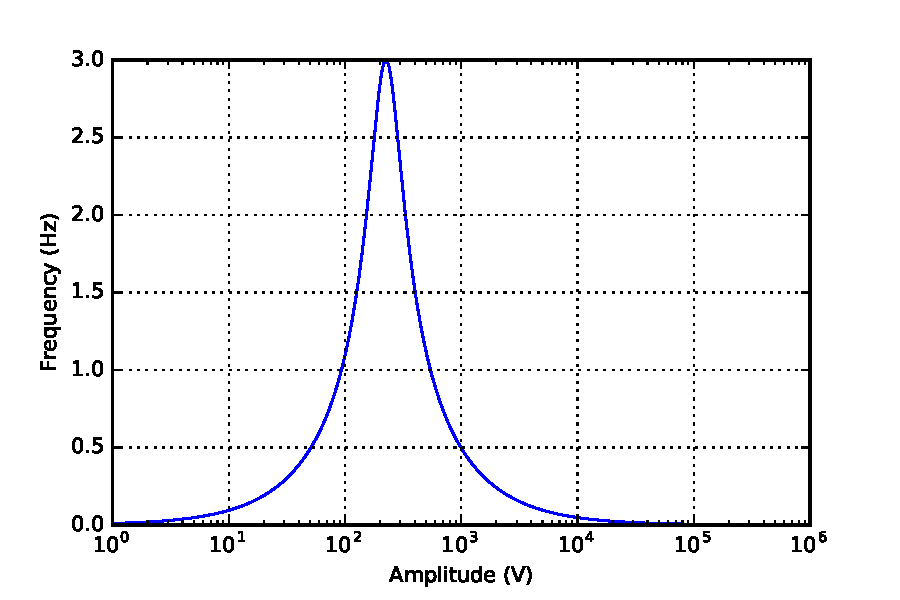
\includegraphics[width=0.5\linewidth]{band-pass-plot.pdf}
\end{figure}
\let\thefootnote\relax\footnote{La mayor\'ia del trabajo algebr\'aico fue realizado en Python usando computaci\'on simb\'olica. \href{https://github.com/jsbarbosa/study-happiness/blob/master/Electronica/Laboratorios/Practica\%208/Preinforme\%208.ipynb}{https://github.com/jsbarbosa/study-happiness/blob/master/Electronica/Laboratorios/Practica\%208/Preinforme\%208.ipynb}}
\end{document}
